\subsubsection{Registration using a Facebook account.}

	To accompany this diagram, read the Scenario \hyperref[sec:FacebookCustomerRegistrationScenario]{S.2}.

				\begin{table}[htpb]
					\centering
					\label{tab:FacebookCustomerRegistrationDiagramTable}
					\begin{tabularx}{\textwidth}{ll}
						\hline
						\hline
							\textbf{Subject}
						& 
							\textbf{Description}\\
						\hline
							Actors	       &  Guest User, myTaxiService Application, \\
							               &  myTaxiService Server, Facebook Login System\\
						\hline
							Preconditions  &  Guest User must not be already registered\\
						\hline
							Execution      &  1.~Guest User open the myTaxiService Application.\\
										   &  2.~Guest User taps on the "Log in with Facebook" button.\\
										   &  3.~myTaxiService Application calls Facebook Login API\\
										   &  4.~Facebook Login System makes his stuff\\
										   &  5.~Facebook Login System reply\\
										   &  6.~myTaxiService Application shows the result to the \\
										   &     Guest User\\
						\hline
							Postconditions &  The Guest User is now a Customer, he is registered in \\ 
										   &  the database and he's now logged in.\\
						\hline
							Exceptions     &  1.~The connection is lost or the Guest User doesn't complete\\ 
										   &     the registration clicking the button.\\
									
						\hline
						\hline
					\end{tabularx}
				\end{table}
				\begin{center}
					%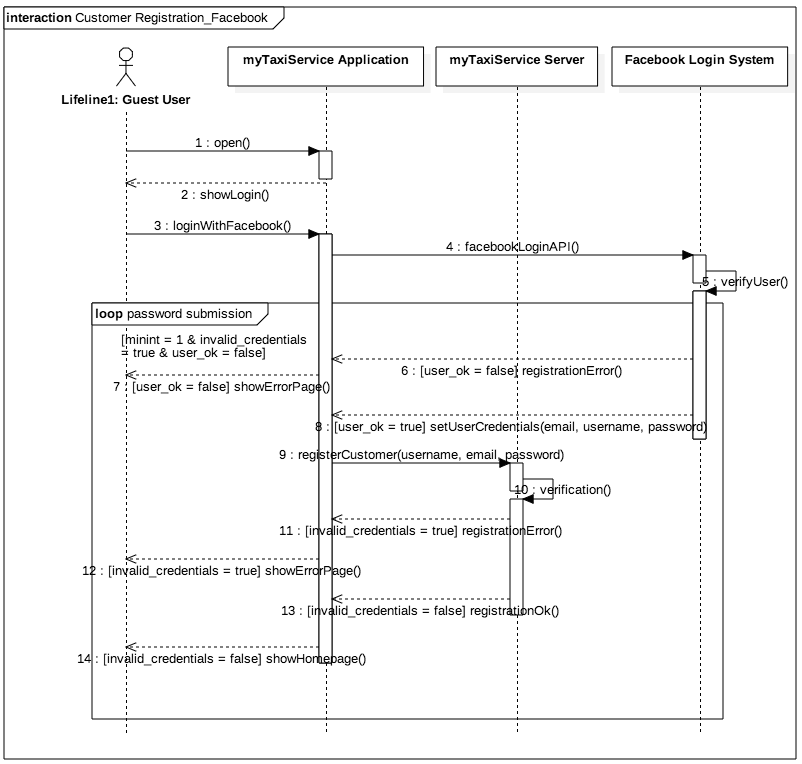
\includegraphics[scale=0.5]{IMG/InteractionDiagrams/CustomerRegistration_Facebook.png}
				\end{center}